\section{zmq-broker}

\begin{figure}
\centering
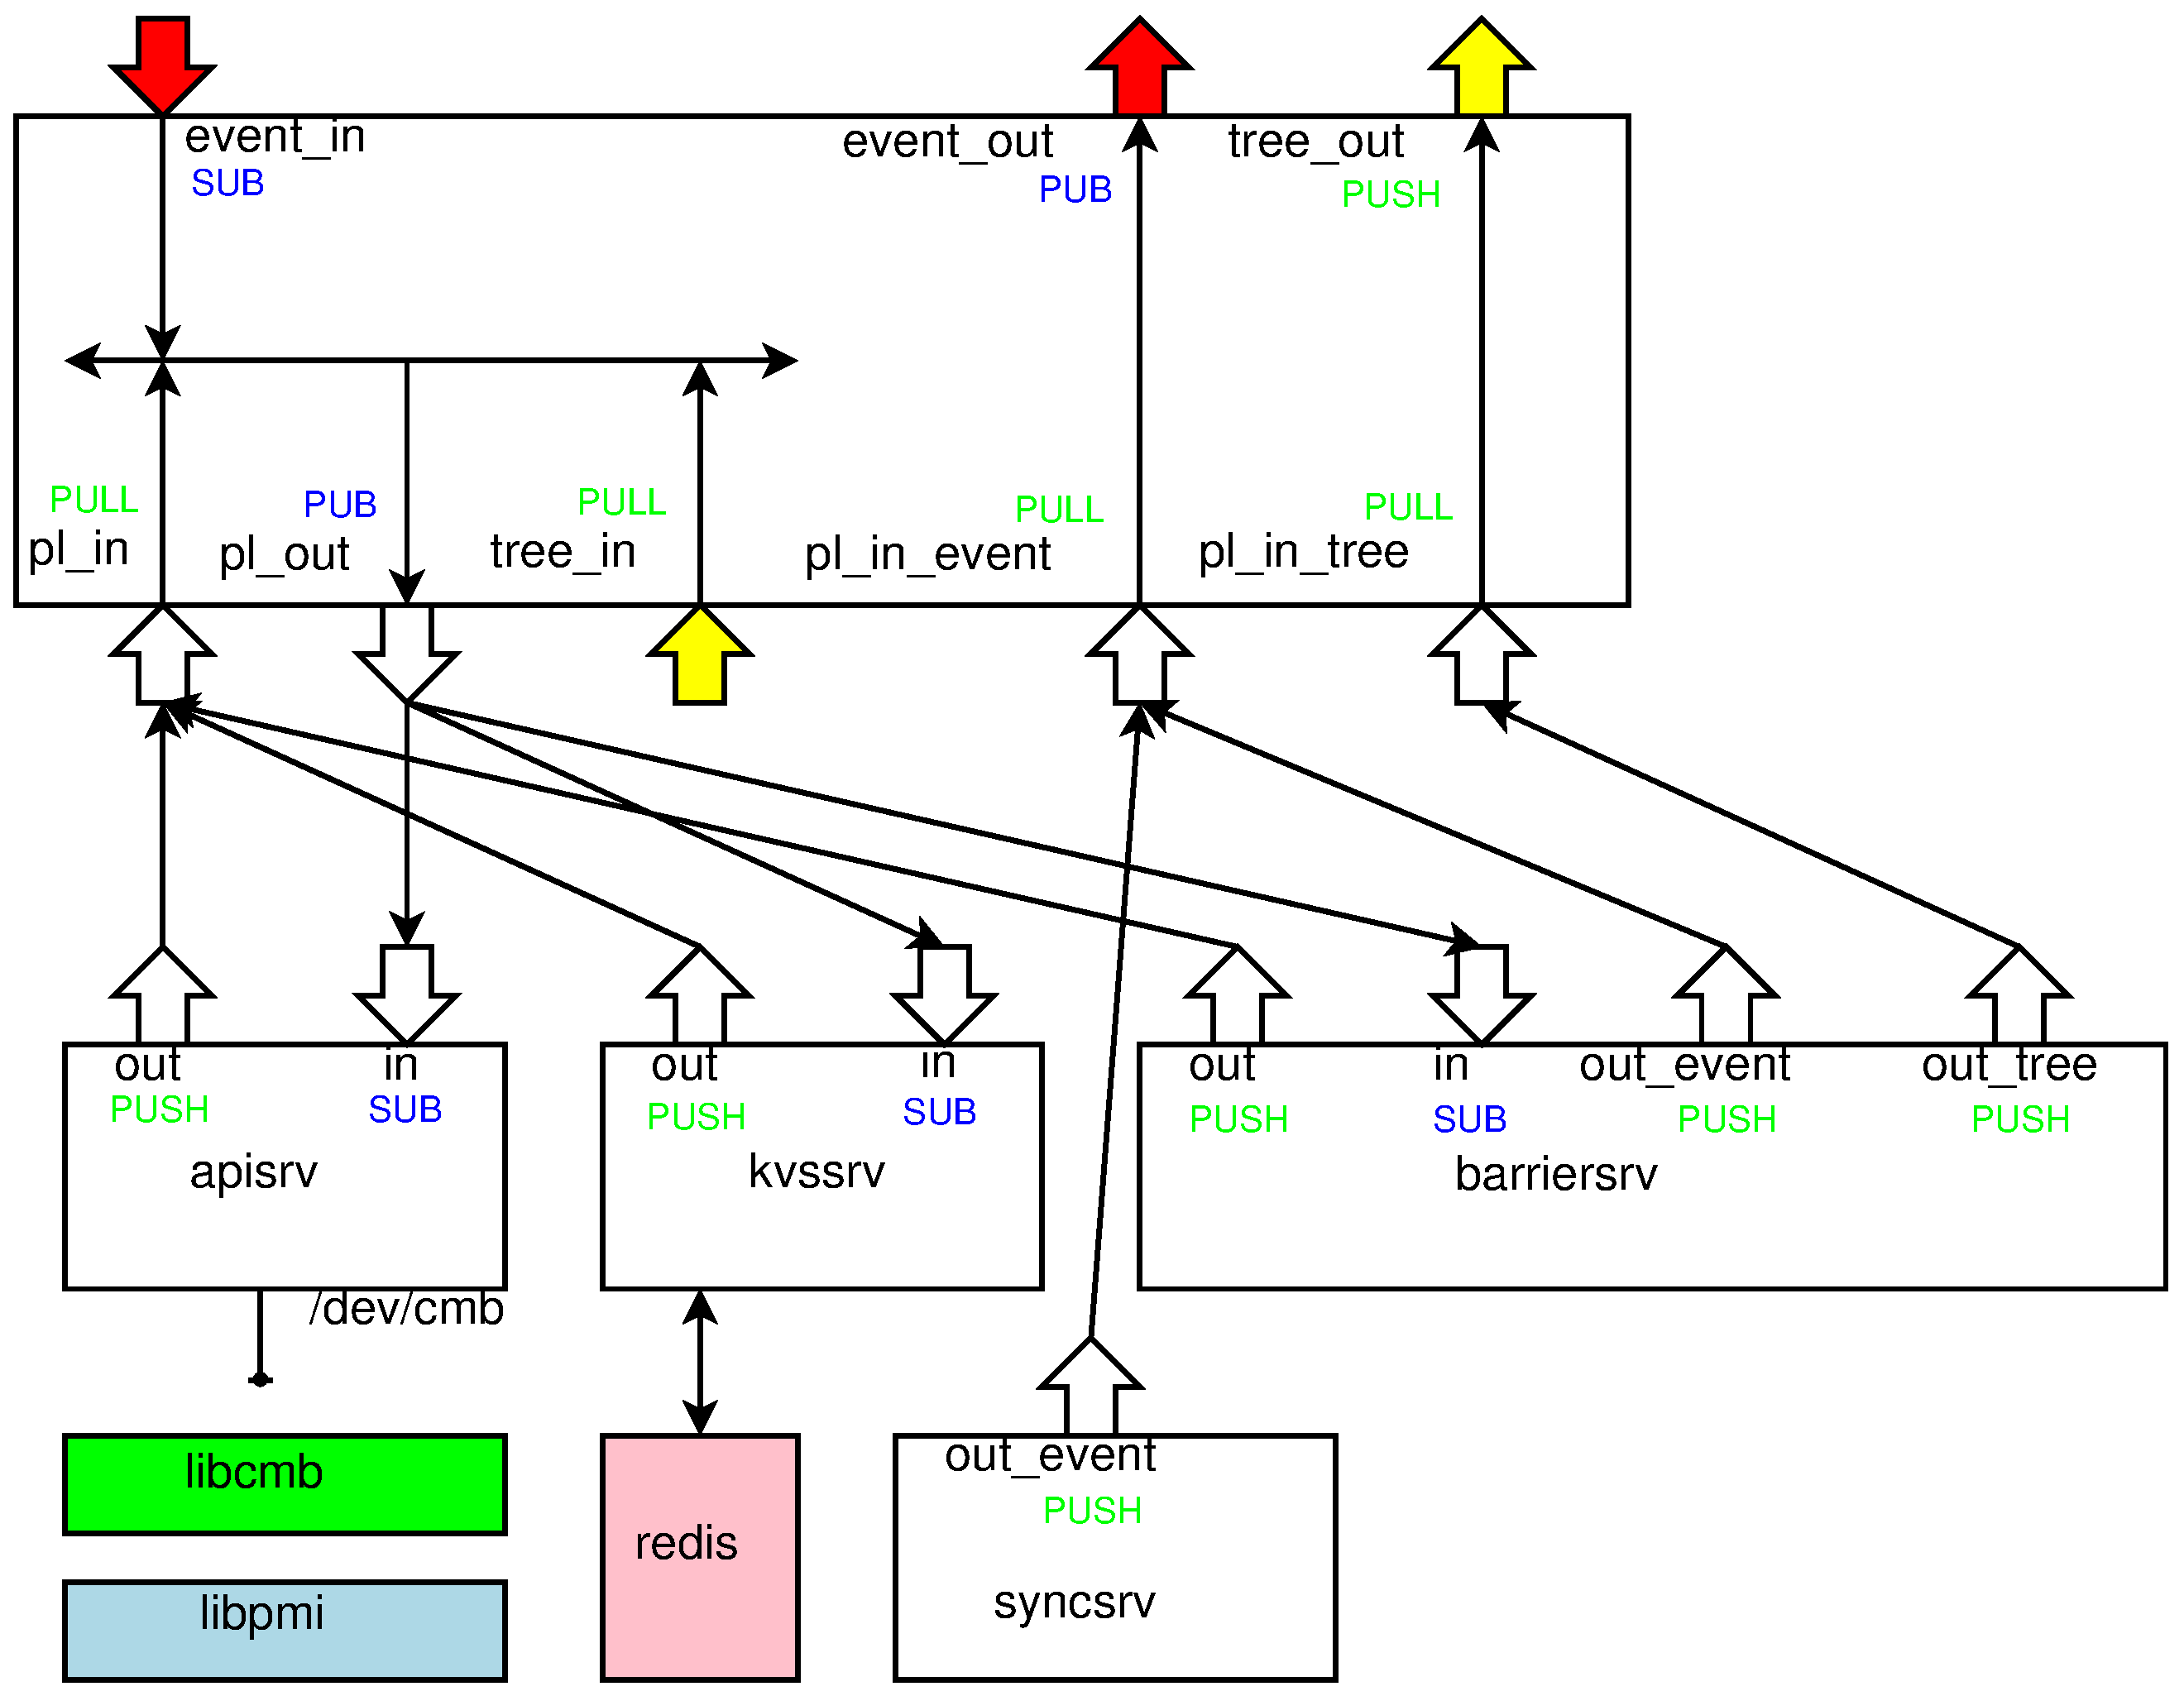
\includegraphics[scale=0.30]{zmq-broker.eps}
\caption{Broker internal architecture.  The cmbd simply routes messages
between \zMQ\ sockets, while plugins (syncsrv, apisrv, kvssrv, barriersrv)
perform specialized services.
Plugins are implemented as threads spawned by the cmbd, and communicate
with the cmbd using {\em inproc} (shared memory) \zMQ\ sockets.
The {\em libcmb} library, which provides the system's public interfaces,
communicates with the broker via a UNIX domain socket.}
\label{fig:cmbinternal}
\end{figure}

\begin{table}
\centering
\begin{tabular}{|l|l|l|l|}\hline
\textbf{Plugin-sock} & \textbf{CMB-sock} & \textbf{CMB-sock} & External \\
\hline
out (PUSH)		& pl\_in (PULL)	& {\em BUS} & \\
out\_event (PUSH)  & pl\_in\_event (PULL) & event\_out (PUB) & $\rightarrow$ \\
out\_tree (PUSH) & pl\_in\_tree	(PULL) & tree\_out (PUSH) & $\rightarrow$ \\
in (SUB)	& pl\_out (PUB)	& {\em BUS}     & \\
\hline
		& {\em BUS}	& event\_in (SUB) & $\leftarrow$ \\
		& {\em BUS}	& tree\_in (PULL) & $\leftarrow$ \\
\hline
\end{tabular}
\caption{The cmbd internal routing table.}
\label{fig:cmbrouting}
\end{table}


